% =====================================================================
%  IEEE conference paper
%  Digital-Twin-Driven Hybrid ANN--ANFIS Task Offloading for
%  Solar-Powered IoT Edge Nodes
%
%  Compile:  pdflatex main.tex  (run twice for references)
%  Figures:  ./figures/*.png  (generated from the project code)
% =====================================================================
\documentclass[conference]{IEEEtran}
\IEEEoverridecommandlockouts

\usepackage{cite}
\usepackage{amsmath,amssymb,amsfonts}
\usepackage{graphicx}
\usepackage{booktabs}
\usepackage{multirow}
\usepackage{algorithm}
\usepackage{algpseudocode}
\usepackage{xcolor}
\usepackage{url}
\graphicspath{{figures/}}

\newcommand{\Jl}{J_{\mathrm{loc}}}
\newcommand{\Jo}{J_{\mathrm{off}}}

\begin{document}

\title{A Digital-Twin-Driven Hybrid ANN--ANFIS Framework for Explainable, Renewable-Aware Task Offloading in Solar-Powered IoT Edge Nodes}

% ---- Replace with the final author list and affiliations ----------------
\author{
\IEEEauthorblockN{Rohith Sivakumar}
\IEEEauthorblockA{\textit{Department of Electrical and Electronics Engineering} \\
\textit{Institution Name}\\
City, Country \\
rohithsivakumar1205@gmail.com}
\and
\IEEEauthorblockN{Second Author}
\IEEEauthorblockA{\textit{Department Name} \\
\textit{Institution Name}\\
City, Country \\
email@domain.com}
}

\maketitle

% =====================================================================
\begin{abstract}
Battery-constrained Internet of Things (IoT) nodes powered by small photovoltaic (PV) panels must decide, task by task, whether
to compute locally or to offload computation to an edge server over a fluctuating wireless link. The best choice depends on the
state of charge (SOC), the task size and complexity, the link quality and the edge server load. Optimal decisions require the
true offload latency and energy, which are unknown before transmission. This paper presents a physics-based, closed-loop
digital twin of a solar-powered ESP32 node that couples a stochastic PV model, a Li-ion battery energy balance, an IEEE~802.11n
rate-adaptation and packet-error model with MQTT/TCP overhead, and an M/M/1 edge server. A battery-risk energy price
$\lambda(\mathrm{SOC})$ makes the offloading behaviour emerge from physics rather than from fixed rules. Using the twin's exact
cost comparison as an oracle teacher, we propose a \emph{predict-then-reason} hybrid controller. A multilayer perceptron (ANN)
predicts the unknown offload time and energy from information available at decision time, and an Adaptive Neuro-Fuzzy Inference
System (ANFIS) with 36 learned Takagi--Sugeno rules converts these predictions into an explainable offload decision. On an unseen
simulated week in closed loop, the hybrid agrees with the oracle in 96.6\% of the decisions, against 92.7\% for an expert Mamdani
fuzzy controller and 95.9\% for a black-box ANN classifier. It reduces task energy by 4.7\% and 2.1\% respectively, cuts deadline
misses by 44\% relative to the fuzzy controller, and provides a rule-level explanation for every decision.
\end{abstract}

\begin{IEEEkeywords}
digital twin, computation offloading, edge computing, energy harvesting, IoT, ANFIS, fuzzy logic, neural network, explainable AI
\end{IEEEkeywords}

% =====================================================================
\section{Introduction}
Edge computing moves computation close to IoT devices to reduce latency and device energy~\cite{shi2016edge,mao2017survey}.
For a battery-limited node, \emph{computation offloading}, that is, executing a task on an edge server instead of locally, can save
energy and time. It is not free, however: data must be transmitted over a wireless link whose rate, packet error rate and
retransmissions depend on the signal strength, and the edge server may be congested. When the node harvests energy from a small
PV panel, the value of energy itself changes over time with the battery state of charge~\cite{mao2016dynamic,huang2020drl}.

Intelligent controllers based on fuzzy logic, artificial neural networks (ANN) and ANFIS have long been used to manage
renewable energy systems. Hemanand~\emph{et~al.}~\cite{hemanand2018comparative} compared fuzzy, ANN and ANFIS controllers for the
maximum power point tracking and microgrid integration of a hybrid PV/wind system, and Muthukumar~\emph{et~al.}~\cite{muthukumar2024comparative}
reviewed intelligent control methodologies for bidirectional power converters in electric mobility. In edge computing, fuzzy
workload orchestrators~\cite{sonmez2019fuzzy,nguyen2020flexible} capture the intuition of human administrators, and deep
learning approaches~\cite{huang2020drl} learn offloading policies from data. Three gaps remain:
\begin{enumerate}
  \item Most offloading studies abstract the energy source and the physical link. Few close the loop in which each decision drains
        a PV-charged battery that conditions all future decisions.
  \item Many formulations implicitly assume that the offload latency and energy are known when the decision is taken, which is not
        true for a real node before it transmits.
  \item Accurate learned policies are usually black boxes, while interpretable fuzzy controllers rely on hand-tuned membership
        functions.
\end{enumerate}

Digital twins~\cite{tao2019digital,fuller2020digital} are well suited to these gaps: a physically faithful replica can generate
labelled experience, provide an ideal teacher and evaluate controllers safely in closed loop. The \textbf{contributions} of this
paper are:
\begin{itemize}
  \item A \textbf{physics-based closed-loop digital twin} of a solar-powered ESP32 IoT node. It couples PV generation with
        Ornstein--Uhlenbeck cloud dynamics, a Li-ion energy balance with CC/CV taper, 802.11n MCS adaptation with SNR-dependent
        packet errors and MQTT/TCP overhead, and an M/M/1 edge server. A battery-risk price $\lambda(\mathrm{SOC})$ lets offloading
        behaviour emerge from physics. Twenty automated engineering checks verify the twin.
  \item An \textbf{information-realistic formulation} that separates the oracle (perfect knowledge) from what a node observes at
        decision time (current SOC and task, \emph{last} measured RSSI and \emph{last} reported server load).
  \item A \textbf{predict-then-reason hybrid controller}. An ANN predicts the offload time and energy, and an ANFIS, trained on the
        ANN's \emph{predictions} with a soft oracle-preference target and input-range clipping, turns them into a decision expressed as
        readable IF--THEN rules.
  \item A \textbf{closed-loop comparison} on an unseen week against a Mamdani expert fuzzy controller and an ANN classifier. The
        hybrid is the most oracle-consistent, the most energy-efficient and fully explainable.
\end{itemize}

The rest of the paper is organised as follows. Section~II reviews related work, Section~III presents the twin, Section~IV the
hybrid controller, Section~V the setup and Section~VI the results. Section~VII concludes.

% =====================================================================
\section{Related Work}
\textbf{Computation offloading.} Mobile edge computing surveys~\cite{mao2017survey,shi2016edge} formulate offloading as a trade-off
between transmission and computation costs. Chen~\emph{et~al.}~\cite{chen2016efficient} studied multi-user offloading games, and
Mao~\emph{et~al.}~\cite{mao2016dynamic} addressed dynamic offloading for energy-harvesting devices with Lyapunov optimisation.
Huang~\emph{et~al.}~\cite{huang2020drl} used deep reinforcement learning for wireless-powered MEC. These works assume known
channel gains or idealised links, and their policies are not interpretable.

\textbf{Fuzzy and neuro-fuzzy decision making.} Fuzzy sets~\cite{zadeh1965fuzzy} and Mamdani controllers~\cite{mamdani1975experiment}
encode expert knowledge in linguistic rules. Sonmez~\emph{et~al.}~\cite{sonmez2019fuzzy} proposed fuzzy workload orchestration for
edge computing, and Nguyen~\emph{et~al.}~\cite{nguyen2020flexible} a fuzzy-based mobile edge orchestrator. ANFIS~\cite{jang1993anfis},
built on the Takagi--Sugeno model~\cite{takagi1985fuzzy}, learns membership functions and rule consequents from data. In renewable
energy systems, fuzzy, ANN and ANFIS controllers have been compared for PV/wind MPPT and microgrid
integration~\cite{hemanand2018comparative}, and intelligent control of power converters has been surveyed
in~\cite{muthukumar2024comparative}. To our knowledge, an ANN-predictor--ANFIS-reasoner pipeline trained by a digital-twin oracle has
not been applied to renewable-aware IoT task offloading.

\textbf{Digital twins.} Tao~\emph{et~al.}~\cite{tao2019digital} and Fuller~\emph{et~al.}~\cite{fuller2020digital} review digital
twins as high-fidelity virtual replicas used for monitoring, prediction and decision support. We use the twin both as a data
generator and as an evaluation environment.

% =====================================================================
\section{Digital Twin System Model}
\begin{figure}[t]
\centering
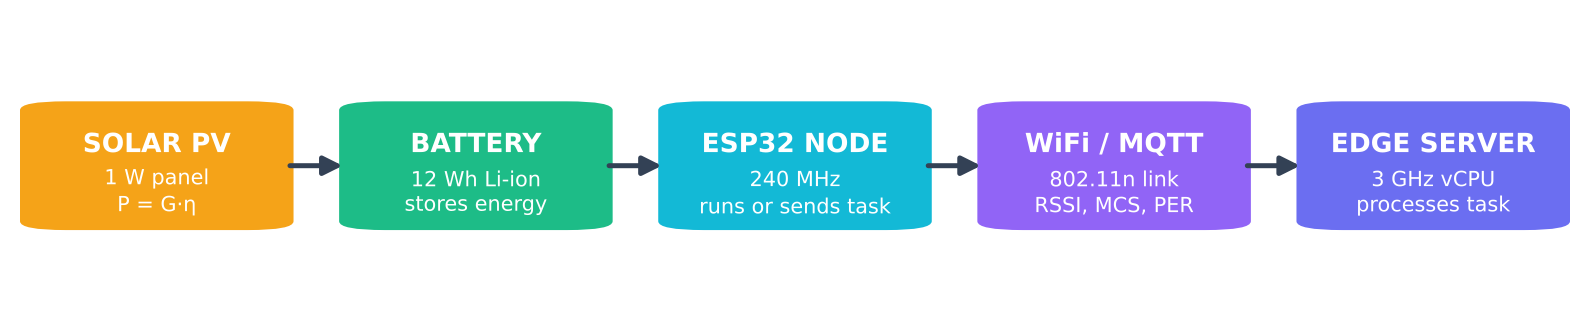
\includegraphics[width=\columnwidth]{chain.png}
\caption{Physical chain mirrored by the digital twin (one task per minute).}
\label{fig:chain}
\end{figure}

The twin (Fig.~\ref{fig:chain}) advances in steps of $\Delta t = 60$\,s. In each step the environment evolves, one task arrives,
both execution options are evaluated with physical models, the cheaper option is selected, and the battery is updated with the energy
of the \emph{chosen} option. Randomness enters only through exogenous physical processes; no noise is added to costs or decisions.

\subsection{PV Generation and Battery}
Clear-sky irradiance follows $G_{\mathrm{clr}}(h)=1000\sin\!\big(\pi(h-6)/12\big)$\,W/m$^2$ for $6<h<18$. Cloud transmittance
$k(t)$ is an Ornstein--Uhlenbeck process around a daily mean (Sunny 0.85, Partly Cloudy 0.60, Overcast 0.30), and the daily weather
follows a Markov chain. The PV power is
\begin{equation}
P_{\mathrm{PV}} = P_{\mathrm{rated}}\,\frac{G_{\mathrm{clr}}\,k}{G_{\mathrm{STC}}}\,\eta_{\mathrm{PV}} .
\end{equation}
With $P_{\mathrm{load}} = P_{\mathrm{base}} + E_{\mathrm{task}}/\Delta t$, the SOC of a battery with capacity $E_{\mathrm{bat}}$ evolves as
\begin{equation}
\mathrm{SOC}^{+} = \mathrm{SOC} + \frac{100\,\Delta t}{E_{\mathrm{bat}}}
\Big(\eta_c P_{\mathrm{ch}} - \frac{P_{\mathrm{dis}}}{\eta_d}\Big),
\end{equation}
where $P_{\mathrm{ch}}=\max(0,P_{\mathrm{PV}}-P_{\mathrm{load}})$ (reduced to 60\% above 90\% SOC, CC/CV taper) and
$P_{\mathrm{dis}}=\max(0,P_{\mathrm{load}}-P_{\mathrm{PV}})$.

\subsection{Task and Local Execution}
A task has data size $D$ (bytes, AR(1) in log-scale with a working-hour activity profile) and complexity $c$ (cycles/byte)
determined by one of five task types (60--3000 cycles/byte). The required cycles are $C=Dc$. With ESP32 clock $f_{\ell}$ and
background load $b$,
\begin{align}
T_{\mathrm{loc}} &= \frac{C}{f_{\ell}(1-b)}, &
E_{\mathrm{loc}} &= \big(P_{\mathrm{idle}}+\alpha\,u\big)\,T_{\mathrm{loc}},
\end{align}
where $u = b + C/(f_{\ell}T_{\mathrm{dl}})$ is the CPU load in percent and $T_{\mathrm{dl}}=5$\,s is the deadline.

\subsection{Wireless Link (802.11n, MQTT over TCP/IP)}
The node--access-point distance $d$ follows a mean-reverting random walk. The RSSI uses the log-distance model with correlated
shadowing~\cite{rappaport2002wireless,gudmundson1991correlation}:
\begin{equation}
\mathrm{RSSI} = \mathrm{RSSI}_0 - 10\,n\log_{10}(d/d_0) + X_\sigma .
\end{equation}
The fastest MCS whose receiver sensitivity $S_m$ is below the RSSI is selected. The packet error rate is
$\mathrm{PER}=1/\big(1+9e^{0.7(\mathrm{RSSI}-S_m)}\big)$ (10\% at sensitivity), the expected number of transmissions is
$N_{\mathrm{tx}}=\min\{1/(1-\mathrm{PER}),7\}$, and the effective rate is $R=R_m\,\eta_{\mathrm{MAC}}(1-U_{\mathrm{ch}})/N_{\mathrm{tx}}$,
where $U_{\mathrm{ch}}$ is channel utilisation by other stations. The uplink time is $T_{\mathrm{tx}}=8B(D)/R$, where $B(\cdot)$ adds
MQTT and per-segment TCP/IP headers.

\subsection{Edge Server}
The edge utilisation $U$ combines a daily usage profile, a slow drift and decaying traffic bursts. Using the M/M/1 sojourn
form~\cite{kleinrock1975queueing}, $T_{\mathrm{edge}} = C/\big(f_e(1-U)\big)$. The total offload time and node energy are
\begin{align}
T_{\mathrm{off}} &= T_{\mathrm{tx}} + T_{\mathrm{res}} + T_{\mathrm{gw}} + T_{q} + T_{\mathrm{edge}},\\
E_{\mathrm{off}} &= P_{\mathrm{tx}}T_{\mathrm{tx}} + P_{\mathrm{rx}}\big(T_{\mathrm{edge}}+T_{\mathrm{res}}+T_{\mathrm{gw}}+T_{q}\big).
\end{align}

\subsection{Battery-Risk Cost and Oracle Decision}
Energy is priced by battery risk,
\begin{equation}
\lambda(\mathrm{SOC}) = 1 + K\,(1-\mathrm{SOC}/100)^{1.5},\qquad K=4,
\end{equation}
and the costs of the two options are
\begin{align}
\Jl &= \lambda\frac{E_{\mathrm{loc}}}{E_{\mathrm{ref}}} + \frac{T_{\mathrm{loc}}}{T_{\mathrm{dl}}} + w_d\,\mathbb{1}[T_{\mathrm{loc}}>T_{\mathrm{dl}}],\\
\Jo &= \lambda\frac{E_{\mathrm{off}}}{E_{\mathrm{ref}}} + \frac{T_{\mathrm{off}}}{T_{\mathrm{dl}}} + w_p\,\mathrm{PER} + w_s U^2 + w_d\,\mathbb{1}[T_{\mathrm{off}}>T_{\mathrm{dl}}],
\end{align}
with $w_d=2$ and $w_p=w_s=0.3$. The \emph{oracle} chooses $\arg\min\{\Jl,\Jo\}$. Because $\lambda$ multiplies both energies, a low SOC
favours offloading when the link is good, but favours local execution when the link is poor, because retransmissions then make the
radio more expensive than the CPU. Solar generation influences decisions only through the SOC.

% =====================================================================
\section{Proposed Hybrid ANN--ANFIS Controller}
\subsection{Decision-Time Observability}
The oracle uses $T_{\mathrm{off}}$, $E_{\mathrm{off}}$ and the current $U$, none of which is known before transmission. A realistic
controller observes only
$\mathbf{o}_t=\{\mathrm{SOC}_t, D_t, c_t, h_t, T_{\mathrm{loc}}, E_{\mathrm{loc}}, \mathrm{RSSI}_{t-1}, U_{t-1}\}$:
the local cost is computable on the device, while the RSSI and the server load are those measured with the \emph{previous} task.
The oracle is therefore used only as a teacher and as the reference for evaluation.

\subsection{Stage 1: ANN Offload-Cost Predictor}
A multilayer perceptron (6--24--16--2, $\tanh$ hidden units, linear output) maps
$\mathbf{x}=[\ln D,\ln c,\mathrm{RSSI}_{t-1},U_{t-1},\sin(2\pi h/24),\cos(2\pi h/24)]$ to
$[\ln \hat T_{\mathrm{off}}, \ln \hat E_{\mathrm{off}}]$. Inputs and targets are standardised. The network is trained with
back-propagation~\cite{rumelhart1986learning} and Adam~\cite{kingma2015adam} on the mean squared error (60 epochs, batch 128).
The logarithmic targets make the network learn relative errors over a range of more than two decades.

\subsection{Stage 2: ANFIS Reasoner}
The ANFIS receives four inputs built from the ANN predictions and the observable state:
\begin{equation}
\mathbf{z} = \Big[\mathrm{SOC},\;
\log_{10}\frac{\hat E_{\mathrm{off}}}{E_{\mathrm{loc}}},\;
100\frac{T_{\mathrm{loc}}-\hat T_{\mathrm{off}}}{T_{\mathrm{dl}}},\;
U_{t-1}\Big],
\end{equation}
with linguistic terms \{Low, Medium, High\}, \{Offload cheaper, Similar, Local cheaper\}, \{Small, Large\} and \{Light, Busy\}.
A grid partition yields $R=3\cdot3\cdot2\cdot2=36$ rules. Following the first-order Takagi--Sugeno model~\cite{takagi1985fuzzy,jang1993anfis},
\begin{align}
\mu_{ij}(z_i) &= \exp\!\Big(-\frac{(z_i-c_{ij})^2}{2\sigma_{ij}^2}\Big), &
w_r &= \prod_{i}\mu_{i,j_r(i)}(z_i),\\
\bar w_r &= \frac{w_r}{\sum_k w_k}, &
y &= \sum_{r=1}^{R}\bar w_r\,(\mathbf{p}_r^\top\mathbf{z}+q_r),
\end{align}
where $y\in[0,1]$ is the offload score and the decision is OFFLOAD if $y>0.5$.

\textbf{Soft oracle target.} Instead of hard labels, ANFIS regresses the soft preference
\begin{equation}
y^\ast = 0.5 + 0.5\tanh\!\big((\Jl-\Jo)/\tau\big),\qquad \tau=0.25,
\end{equation}
which encodes \emph{how clearly} one option is better. This suits the linear consequents and improved validation accuracy in our
experiments.

\textbf{Hybrid learning.} Each epoch alternates (i) a forward pass, in which the premise parameters $(c,\sigma)$ are fixed and all
consequents $(\mathbf{p}_r,q_r)$ are obtained by ridge least squares, and (ii) a backward pass, in which the consequents are fixed and
$(c,\sigma)$ are updated by gradient descent on the MSE~\cite{jang1993anfis}.

\textbf{Robustness.} The ANFIS is trained on the ANN's \emph{predicted} features, not the true ones, so the rules absorb the
predictor's errors. Inputs are clipped to the training range at inference, which prevents the linear consequents from
extrapolating when the SOC leaves the range seen in training.

\begin{algorithm}[t]
\caption{Predict-then-reason offloading decision}
\label{alg:hybrid}
\begin{algorithmic}[1]
\Require observation $\mathbf{o}_t$, trained ANN $g$, trained ANFIS $F$
\State $(\hat T_{\mathrm{off}},\hat E_{\mathrm{off}}) \gets g(D_t,c_t,\mathrm{RSSI}_{t-1},U_{t-1},h_t)$ \Comment{predict}
\State build $\mathbf{z}$ from $\mathrm{SOC}_t$, $\hat E_{\mathrm{off}}/E_{\mathrm{loc}}$, $(T_{\mathrm{loc}}-\hat T_{\mathrm{off}})/T_{\mathrm{dl}}$, $U_{t-1}$
\State clip $\mathbf{z}$ to the training range
\State $y \gets F(\mathbf{z})$; record the rules with the largest $\bar w_r$ \Comment{reason}
\State \Return OFFLOAD if $y>0.5$ else LOCAL \Comment{decide}
\end{algorithmic}
\end{algorithm}

\begin{figure*}[t]
\centering
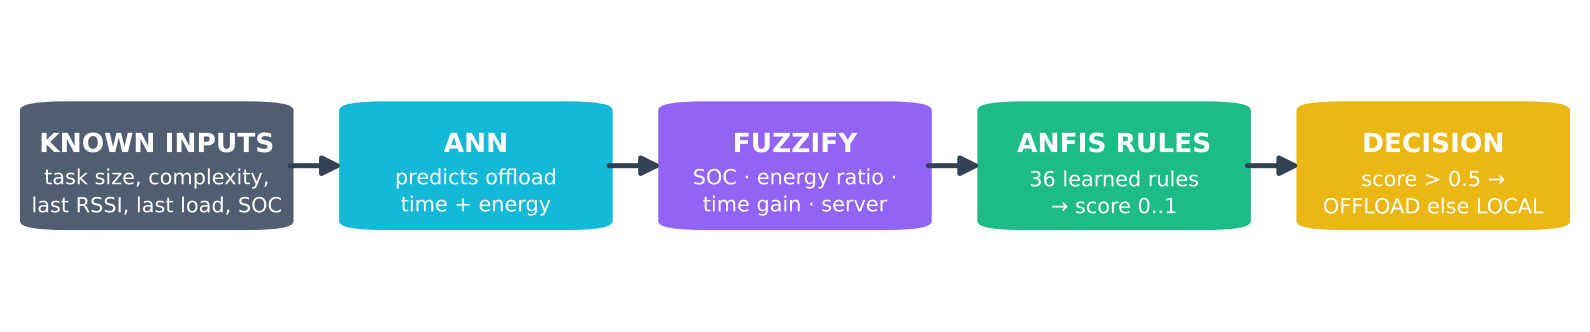
\includegraphics[width=0.92\textwidth]{hybrid.png}
\caption{Proposed predict-then-reason pipeline: the ANN estimates the unknown offload cost and the ANFIS converts it into an explainable decision.}
\label{fig:hybrid}
\end{figure*}

\subsection{Baselines}
\textbf{Oracle:} exact $\arg\min\{\Jl,\Jo\}$ with perfect knowledge (upper bound).
\textbf{Fuzzy only:} a Mamdani controller~\cite{mamdani1975experiment} with inputs SOC, local execution time, $\mathrm{RSSI}_{t-1}$
and $U_{t-1}$ (trapezoidal and triangular sets), 12 expert rules, min--max inference and centroid defuzzification.
\textbf{ANN only:} an MLP classifier (9--24--16--1, sigmoid output, cross-entropy) on the same observations plus SOC and local cost.

% =====================================================================
\section{Simulation Setup}
\begin{table}[t]
\caption{Main Digital-Twin Parameters}
\label{tab:params}
\centering
\footnotesize
\begin{tabular}{@{}ll@{}}
\toprule
Parameter & Value \\
\midrule
PV panel, derating & 1\,W rated, $\eta_{\mathrm{PV}}=0.85$ \\
Battery & 12\,Wh Li-ion, $\eta_c=\eta_d=0.95$ \\
Base load & 0.14\,W (sensors + WiFi association) \\
ESP32 clock, idle power & 240\,MHz, 0.10\,W, $\alpha=0.0012$\,W/\% \\
Task deadline $T_{\mathrm{dl}}$ & 5\,s \\
Path loss & $\mathrm{RSSI}_0=-40$\,dBm, $n=2.6$, $\sigma=4$\,dB \\
802.11n MCS & MCS0--7 (6.5--65\,Mb/s), $\eta_{\mathrm{MAC}}=0.35$ \\
Radio power & $P_{\mathrm{tx}}=0.60$\,W, $P_{\mathrm{rx}}=0.33$\,W \\
Edge server & 3\,GHz vCPU, $U\le 97\%$ \\
Cost weights & $K=4$, $w_d=2$, $w_p=w_s=0.3$ \\
\bottomrule
\end{tabular}
\end{table}

The twin was implemented in Python and NumPy. The ANN, the Mamdani system and the ANFIS were written from first principles in
NumPy, without machine-learning libraries. Table~\ref{tab:params} lists the main parameters. A 7-day run (seed 42, initial SOC 25\%)
produced 10{,}080 labelled tasks: 54.0\% LOCAL and 46.0\% OFFLOAD oracle decisions, with SOC between 15.2\% and 57.4\%. Twenty
automated checks confirmed the expected physical relationships, among them distance~$\uparrow\Rightarrow$~RSSI~$\downarrow$
(Spearman $\rho=-0.78$), server load~$\uparrow\Rightarrow$ edge time per cycle~$\uparrow$ ($\rho=1.00$), energy-balance closure
(error $<10^{-4}\%$) and decision $=\arg\min$ cost (100\%).

The data were split chronologically: the first 80\% for training and the last 20\% (about 1.4 days) for validation. For the
closed-loop test, each controller then drove the battery of the twin for a \emph{new} 7-day week (seed 7) that was never used
in training.

% =====================================================================
\section{Results and Discussion}
\subsection{Prediction Accuracy}
On the validation days, the ANN predicts the offload time with $R^2=0.989$ (median absolute error 5.2\%) and the offload energy
with $R^2=0.987$ (median error 5.6\%), despite observing only the lagged RSSI and server load (Fig.~\ref{fig:ann}).

\begin{figure*}[t]
\centering
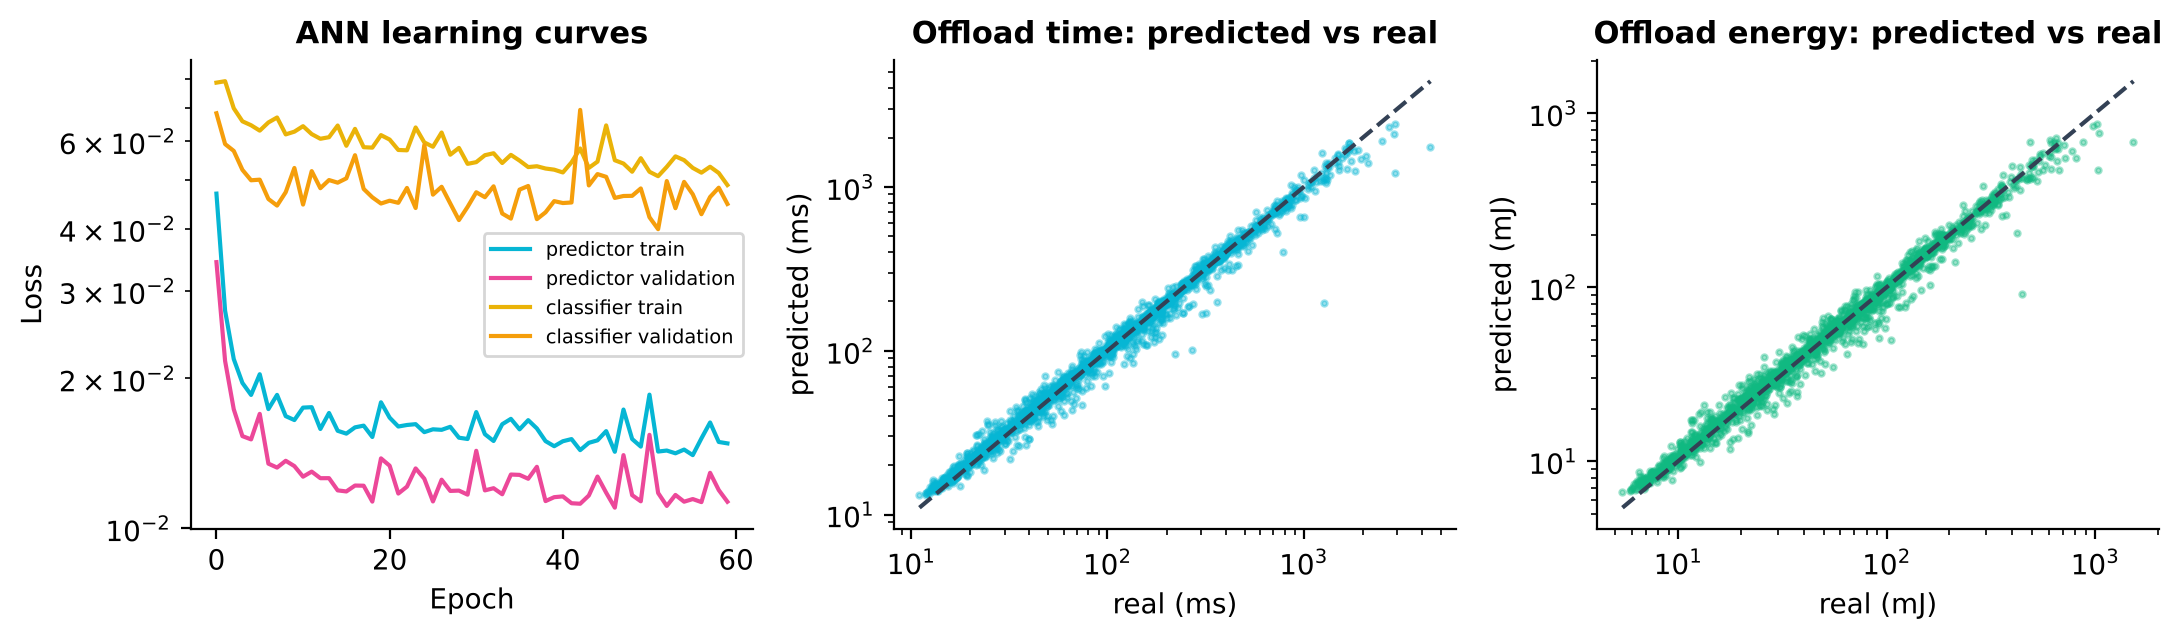
\includegraphics[width=0.95\textwidth]{ann.png}
\caption{ANN learning curves (left) and predicted versus true offload time and energy on validation data (log scales).}
\label{fig:ann}
\end{figure*}

\subsection{Learned Fuzzy Partitions}
Fig.~\ref{fig:anfis} shows the membership functions learned by ANFIS. The energy-ratio partition places ``Similar'' around
$\log_{10}(\hat E_{\mathrm{off}}/E_{\mathrm{loc}})\approx0.4$, which shows that offloading must be clearly cheaper in energy to win
once its risk terms are counted. The most used learned rules on the validation days include
\emph{IF SOC is High $\wedge$ Energy is Similar $\wedge$ Time gain is Small $\wedge$ Server is Busy THEN LOCAL} (14.2\% of the
total firing strength) and \emph{IF SOC is High $\wedge$ Energy is Offload cheaper $\wedge$ Time gain is Large $\wedge$ Server is
Light THEN OFFLOAD}. Both are consistent with engineering intuition.

\begin{figure*}[t]
\centering
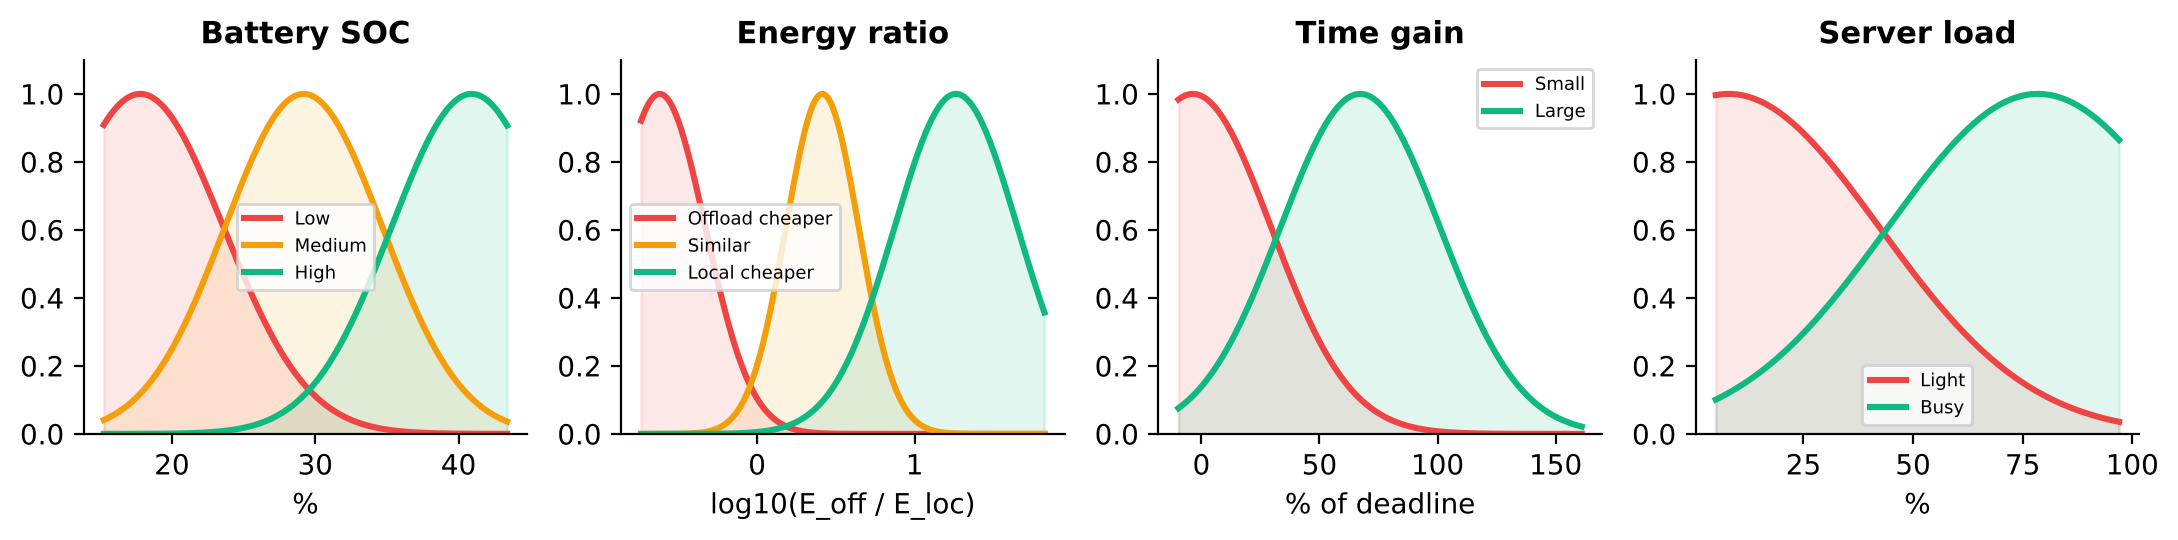
\includegraphics[width=0.95\textwidth]{anfis_mfs.png}
\caption{Gaussian membership functions learned by ANFIS for its four inputs. Ranges correspond to the training data; inputs outside them are clipped.}
\label{fig:anfis}
\end{figure*}

\subsection{Offline and Closed-Loop Performance}
Table~\ref{tab:results} summarises the results. Offline, the ANN classifier and the hybrid reach similar accuracy (98.1\%), clearly
above the expert fuzzy controller (94.8\%). In closed loop on the unseen week, where errors accumulate through the battery, the
hybrid is the most oracle-consistent controller (96.6\%). It also spends the least task energy: 931.8\,J, which is 4.7\% less than
fuzzy-only and 2.1\% less than ANN-only. Its excess energy over the oracle is 20.4\,J, about half that of the ANN (39.9\,J) and less
than a third of the fuzzy controller (66.3\,J). The hybrid misses 9 deadlines, against 11 and 16, and has the lowest mean regret,
0.0097 against 0.0149 and 0.0250 (Fig.~\ref{fig:compare}). Its mean task time is slightly higher than that of the ANN classifier,
because it trades a few milliseconds for energy when the battery price is high. This is the behaviour encoded by the oracle cost.

\begin{table}[t]
\caption{Controller Comparison (Validation Days and Unseen Closed-Loop Week)}
\label{tab:results}
\centering
\footnotesize
\setlength{\tabcolsep}{3.2pt}
\begin{tabular}{@{}lccccc@{}}
\toprule
 & Offline & \multicolumn{4}{c}{Closed loop, unseen week} \\
\cmidrule(lr){2-2}\cmidrule(l){3-6}
Controller & Acc.\,(\%) & Agree.\,(\%) & Energy (J) & Misses & Regret \\
\midrule
Oracle         & 100   & 100   & 911.4 & 0  & 0      \\
Fuzzy only     & 94.84 & 92.70 & 977.8 & 16 & 0.0250 \\
ANN only       & 98.12 & 95.94 & 951.4 & 11 & 0.0149 \\
\textbf{ANN+ANFIS} & \textbf{98.07} & \textbf{96.56} & \textbf{931.8} & \textbf{9} & \textbf{0.0097} \\
\bottomrule
\end{tabular}
\end{table}

\begin{figure*}[t]
\centering
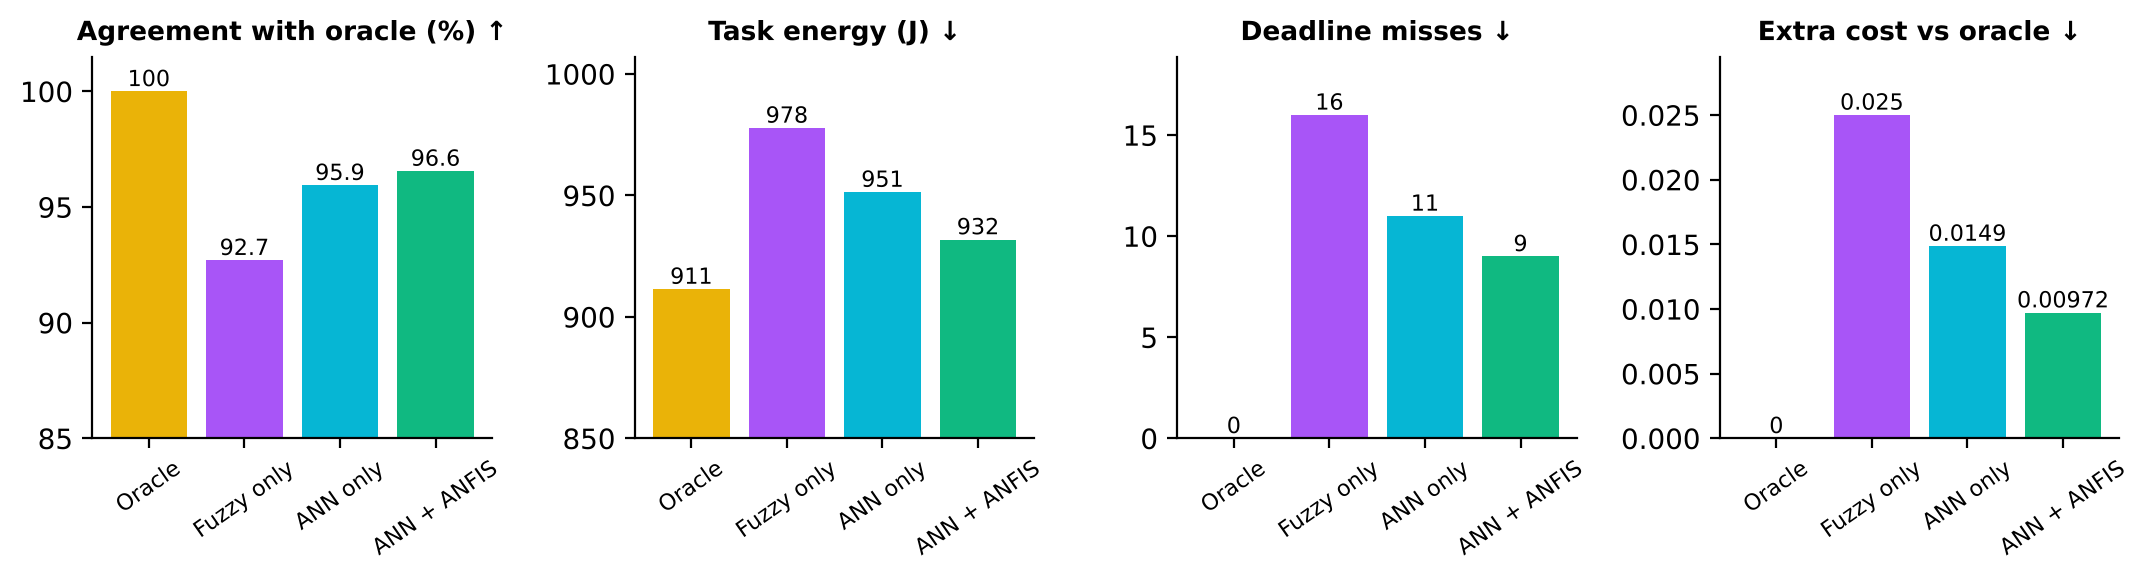
\includegraphics[width=0.95\textwidth]{compare.png}
\caption{Closed-loop comparison on the unseen week: agreement with the oracle, task energy, deadline misses and mean regret.}
\label{fig:compare}
\end{figure*}

\subsection{Explainability: A Worked Decision}
Consider minute~754 of the dataset (12:34, partly cloudy). The node has SOC $=27.6\%$ and receives a 105\,KB FFT feature-extraction
task. Locally the task needs 385\,ms and 46\,mJ. The edge is 69\% busy. The ANN predicts $\hat T_{\mathrm{off}}=180$\,ms and
$\hat E_{\mathrm{off}}=83.6$\,mJ (true values 179\,ms and 81.1\,mJ). The dominant ANFIS rule, \emph{SOC Medium $\wedge$ Energy Similar
$\wedge$ Time gain Small $\wedge$ Server Busy}, receives 50\% of the normalised firing strength and outputs 0.03. The final score
$y=0.16$ gives LOCAL, which matches the oracle ($\Jl=0.237<\Jo=0.483$). The decision is therefore accompanied by a human-readable
justification: offloading would be faster, but it costs about $1.8\times$ the energy while the battery is low and the server is busy.
The black-box ANN classifier reaches the same decision but cannot provide this reasoning.

\subsection{Complexity}
The predictor has 602 parameters and the ANFIS 200 (20 premise and 180 consequent). One decision takes about 0.15\,ms in
unoptimised Python, and the memory footprint is a few kilobytes, which is compatible with on-device execution on the ESP32.

\subsection{Limitations}
The parameters are datasheet-level approximations, WiFi and MQTT are modelled analytically rather than packet by packet, and a single
node is considered. The fuzzy terms of ANFIS are relative to the SOC range seen in training (15--57\%), which motivates training on
more diverse weeks.

% =====================================================================
\section{Conclusion and Future Work}
This paper presented a physics-based closed-loop digital twin of a solar-powered IoT node and a predict-then-reason hybrid controller
for renewable-aware task offloading. Using only information available at decision time, an ANN predicts the offload cost and an ANFIS
converts it into explainable decisions. On an unseen closed-loop week, the hybrid outperformed both an expert fuzzy controller and a
black-box ANN in oracle agreement, energy, deadline misses and regret. Future work will extend the twin to multiple nodes sharing the
channel and the edge, add an ANN solar forecaster as an ANFIS input, support partial offloading driven by the fuzzy score, and
validate the controller on ESP32 hardware with a real MQTT broker.

% =====================================================================
\begin{thebibliography}{99}

\bibitem{shi2016edge}
W.~Shi, J.~Cao, Q.~Zhang, Y.~Li, and L.~Xu, ``Edge computing: Vision and challenges,''
\emph{IEEE Internet Things J.}, vol.~3, no.~5, pp.~637--646, Oct. 2016.

\bibitem{mao2017survey}
Y.~Mao, C.~You, J.~Zhang, K.~Huang, and K.~B. Letaief, ``A survey on mobile edge computing: The communication perspective,''
\emph{IEEE Commun. Surveys Tuts.}, vol.~19, no.~4, pp.~2322--2358, 2017.

\bibitem{mao2016dynamic}
Y.~Mao, J.~Zhang, and K.~B. Letaief, ``Dynamic computation offloading for mobile-edge computing with energy harvesting devices,''
\emph{IEEE J. Sel. Areas Commun.}, vol.~34, no.~12, pp.~3590--3605, Dec. 2016.

\bibitem{huang2020drl}
L.~Huang, S.~Bi, and Y.-J.~A. Zhang, ``Deep reinforcement learning for online computation offloading in wireless powered
mobile-edge computing networks,'' \emph{IEEE Trans. Mobile Comput.}, vol.~19, no.~11, pp.~2581--2593, Nov. 2020.

\bibitem{chen2016efficient}
X.~Chen, L.~Jiao, W.~Li, and X.~Fu, ``Efficient multi-user computation offloading for mobile-edge cloud computing,''
\emph{IEEE/ACM Trans. Netw.}, vol.~24, no.~5, pp.~2795--2808, Oct. 2016.

\bibitem{hemanand2018comparative}
T.~Hemanand, N.~P. Subramaniam, and M.~Venkateshkumar, ``Comparative analysis of intelligent controller based microgrid integration
of hybrid PV/wind power system,'' \emph{J. Ambient Intell. Humaniz. Comput.}, 2018, doi: 10.1007/s12652-018-0961-6.

\bibitem{muthukumar2024comparative}
P.~Muthukumar, M.~Venkateshkumar, and C.~S. Chin, ``A comparative study of cutting-edge bi-directional power converters and
intelligent control methodologies for advanced electric mobility,'' \emph{IEEE Access}, vol.~12, pp.~28710--28752, 2024,
doi: 10.1109/ACCESS.2024.3360267.

\bibitem{sonmez2019fuzzy}
C.~Sonmez, A.~Ozgovde, and C.~Ersoy, ``Fuzzy workload orchestration for edge computing,''
\emph{IEEE Trans. Netw. Service Manag.}, vol.~16, no.~2, pp.~769--782, Jun. 2019.

\bibitem{nguyen2020flexible}
V.~D. Nguyen, T.~T. Khanh, T.~D.~T. Nguyen, C.~S. Hong, and E.-N. Huh, ``Flexible computation offloading in a fuzzy-based mobile edge
orchestrator for IoT applications,'' \emph{J. Cloud Comput.}, vol.~9, art.~66, 2020.

\bibitem{zadeh1965fuzzy}
L.~A. Zadeh, ``Fuzzy sets,'' \emph{Inf. Control}, vol.~8, no.~3, pp.~338--353, 1965.

\bibitem{mamdani1975experiment}
E.~H. Mamdani and S.~Assilian, ``An experiment in linguistic synthesis with a fuzzy logic controller,''
\emph{Int. J. Man-Mach. Stud.}, vol.~7, no.~1, pp.~1--13, 1975.

\bibitem{takagi1985fuzzy}
T.~Takagi and M.~Sugeno, ``Fuzzy identification of systems and its applications to modeling and control,''
\emph{IEEE Trans. Syst., Man, Cybern.}, vol.~SMC-15, no.~1, pp.~116--132, 1985.

\bibitem{jang1993anfis}
J.-S.~R. Jang, ``ANFIS: Adaptive-network-based fuzzy inference system,''
\emph{IEEE Trans. Syst., Man, Cybern.}, vol.~23, no.~3, pp.~665--685, 1993.

\bibitem{rumelhart1986learning}
D.~E. Rumelhart, G.~E. Hinton, and R.~J. Williams, ``Learning representations by back-propagating errors,''
\emph{Nature}, vol.~323, pp.~533--536, 1986.

\bibitem{kingma2015adam}
D.~P. Kingma and J.~Ba, ``Adam: A method for stochastic optimization,'' in \emph{Proc. Int. Conf. Learn. Represent. (ICLR)}, 2015.

\bibitem{tao2019digital}
F.~Tao, H.~Zhang, A.~Liu, and A.~Y.~C. Nee, ``Digital twin in industry: State-of-the-art,''
\emph{IEEE Trans. Ind. Informat.}, vol.~15, no.~4, pp.~2405--2415, Apr. 2019.

\bibitem{fuller2020digital}
A.~Fuller, Z.~Fan, C.~Day, and C.~Barlow, ``Digital twin: Enabling technologies, challenges and open research,''
\emph{IEEE Access}, vol.~8, pp.~108952--108971, 2020.

\bibitem{rappaport2002wireless}
T.~S. Rappaport, \emph{Wireless Communications: Principles and Practice}, 2nd~ed. Upper Saddle River, NJ, USA: Prentice Hall, 2002.

\bibitem{gudmundson1991correlation}
M.~Gudmundson, ``Correlation model for shadow fading in mobile radio systems,''
\emph{Electron. Lett.}, vol.~27, no.~23, pp.~2145--2146, 1991.

\bibitem{kleinrock1975queueing}
L.~Kleinrock, \emph{Queueing Systems, Volume 1: Theory}. New York, NY, USA: Wiley, 1975.

\end{thebibliography}

\end{document}
